\documentclass[12pt]{article}
\usepackage{parskip}
\usepackage{pdfpages}
\usepackage[margin=.6in]{geometry}


\begin{document}
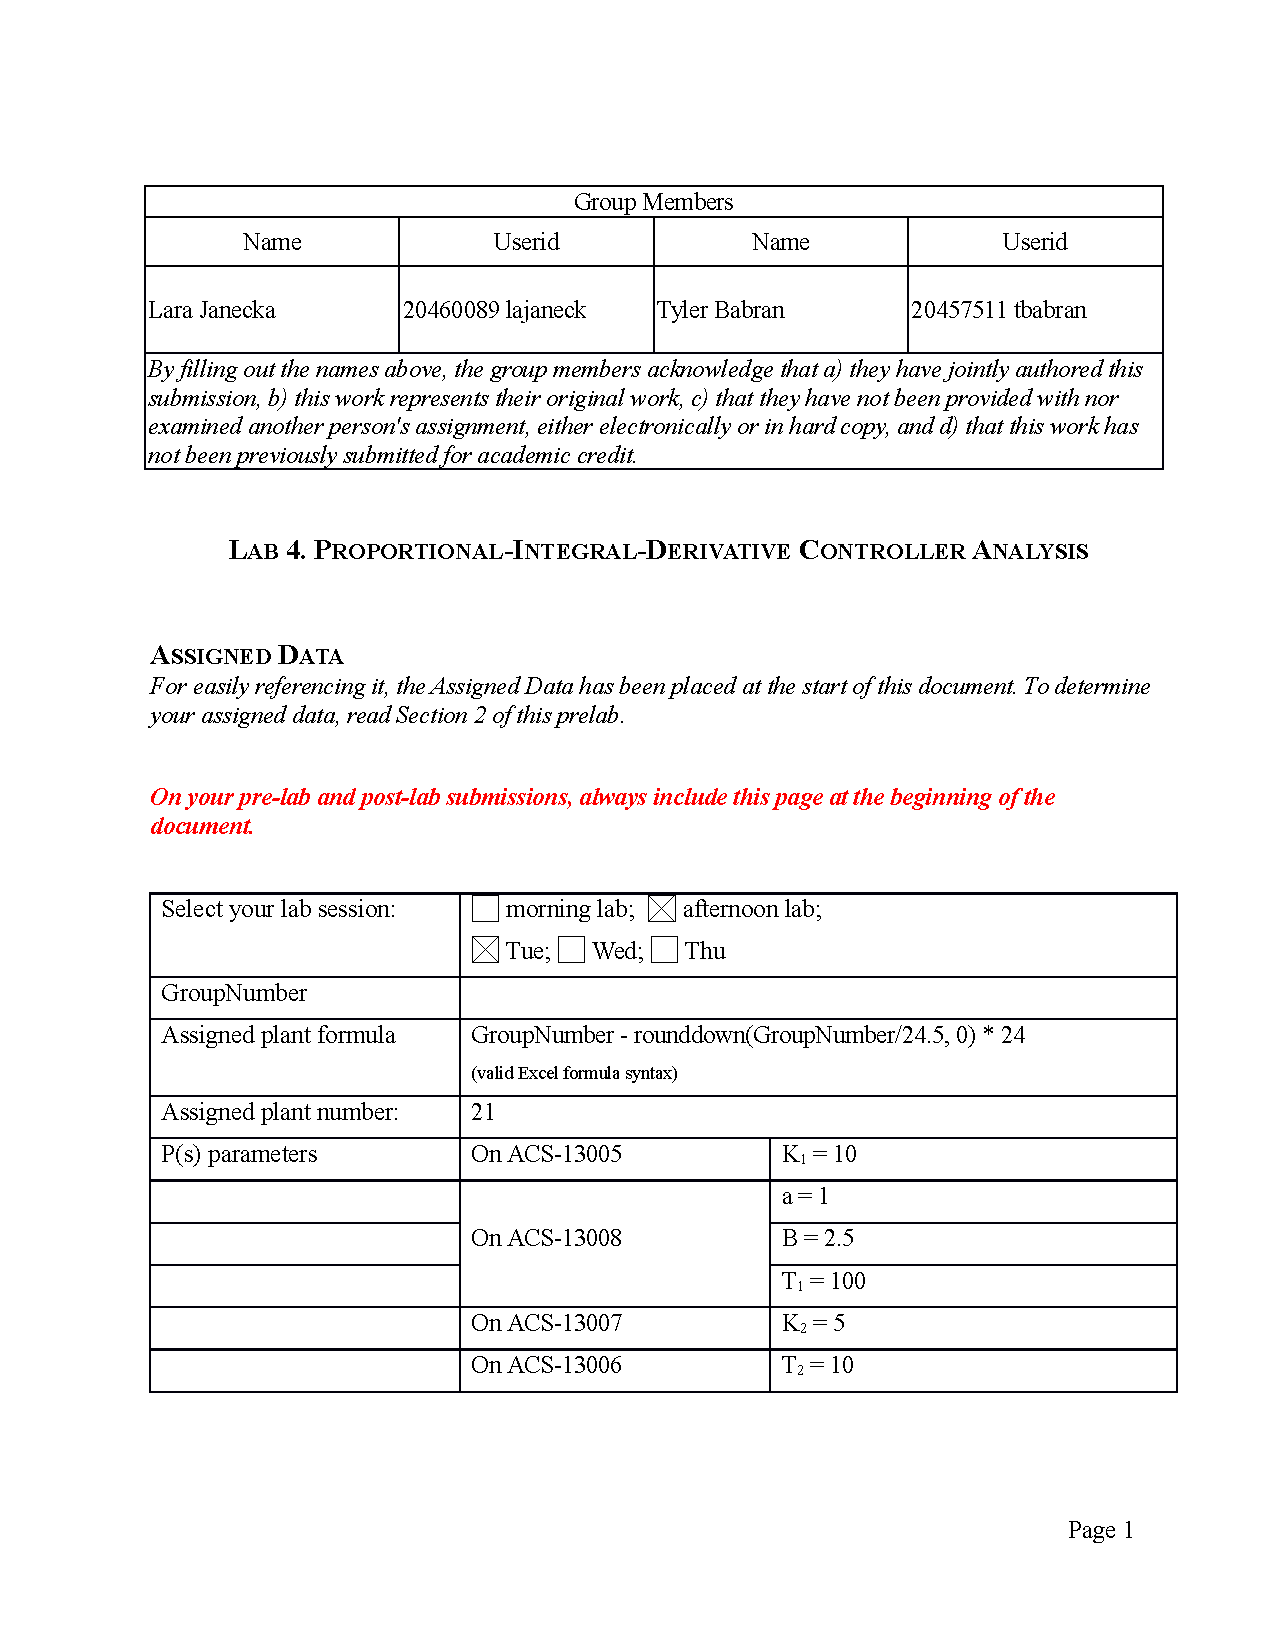
\includepdf{page1}
\begin{table}[ht]
\centering
    \begin{tabular}{|p{2cm}|p{2cm}|p{2cm}|p{2cm}|p{2cm}|p{2cm}|}
        \hline
        \multicolumn{3}{|p{6cm}|}{Measurements at low-frequency} & \multicolumn{3}{|p{6cm}|}{Measurements at bandwidth frequency}\\
        \hline
        \textbf{Peak-to-peak amplitude of output} & \textbf{Frequency (Hz)} & \textbf{Frequency (rad/s)} & \textbf{Peak-to-peak amplitude of output} & \textbf{Frequency (Hz)} & \textbf{Frequency (rad/s)}\\
        \hline
        3  & 10 & 62.8  &  2.11  &  63.69 &  400\\
        \hline
    \end{tabular}
    \caption{Open-loop bandwidth measurements in time domain}
    \label{tab:open-loop}
\end{table}

\paragraph{Bandwidth measuring procedure} % (fold)
\label{par:bandwidth_measuring_procedure}
To measure the bandwidth we first measured the output amplitude at a suitably low frequency (we used 10Hz). From there we calculated what the bandwidth output amplitude should be by dividing the output amplitude at our low frequency by $\sqrt{2}$. After marking this value with a cursor on the graph we altered the input freqency until we reached our calculated output amplitude, this frequency was our bandwidth.
% paragraph bandwidth_measuring_procedure (end)


\begin{table}[ht]
\centering
    \begin{tabular}{|p{2cm}|p{2cm}|p{2cm}|p{2cm}|p{2cm}|p{2cm}|}
        \hline
        \multicolumn{3}{|p{6cm}|}{Measurements at low-frequency} & \multicolumn{3}{|p{6cm}|}{Measurements at bandwidth frequency}\\
        \hline
        \textbf{Peak-to-peak amplitude of output} & \textbf{Frequency (Hz)} & \textbf{Frequency (rad/s)} & \textbf{Peak-to-peak amplitude of output} & \textbf{Frequency (Hz)} & \textbf{Frequency (rad/s)}\\
        \hline
        0.78   & 10&  62.8 &   0.55   & 238.85 & 1500\\
        \hline
    \end{tabular}
    \caption{Closed-loop bandwidth measurements in time domain}
    \label{tab:closed-loop}
\end{table}


\begin{figure}[ht]
\centering
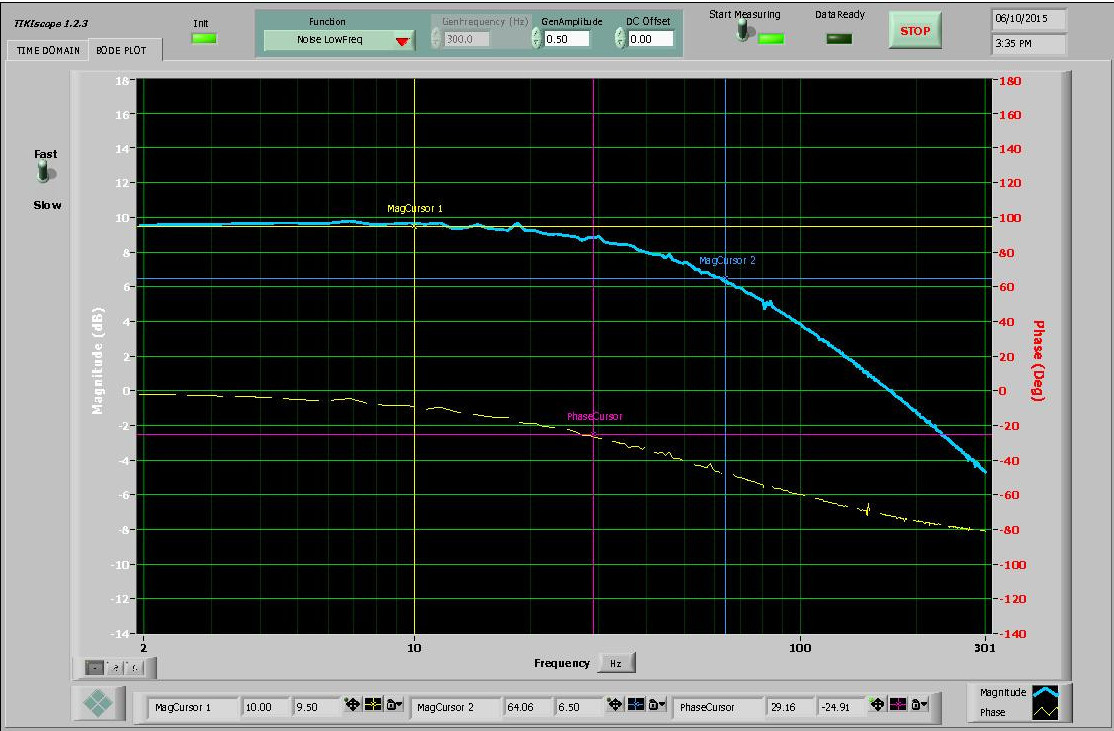
\includegraphics[width=7in]{FreqRespOpen.jpg}
\caption{Open-loop configuration}
\label{fig:open-loop}
\end{figure}

\begin{figure}[ht]
\centering
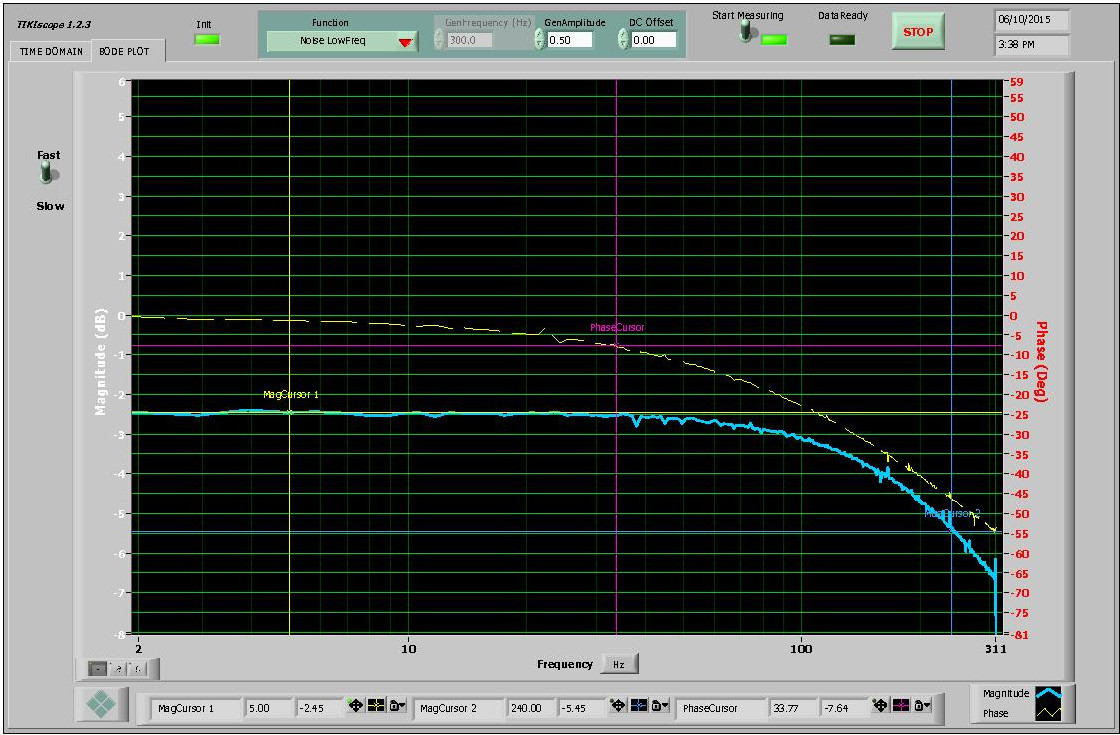
\includegraphics[width=7in]{FreqRespClosed.jpg}
\caption{Closed-loop configuration}
\label{fig:closed-loop}
\end{figure}

\begin{table}[ht]
\centering
    \begin{tabular}{|l|p{2cm}|p{2cm}|p{2cm}|p{2cm}|p{2cm}|p{2cm}|}
        \hline
        & \textbf{Bandwidth in time domain} & \textbf{Bandwidth in freq domain} & \textbf{Bandwidth in Matlab} & \textbf{Bandwidth theoretical} & \textbf{Error Theor TimeDom (\%)} & \textbf{Error Theo FreqDom (\%)}\\
        \hline
        \textbf{Open-loop} & 63.9 & 64 & 65.7 & 63.69 & 0.33\% & 0.49\%\\
        \hline
        \textbf{Closed-loop} & 238.85 & 240 & 246.3 & 238.85 & 0\% & 0.48\%\\
        \hline
    \end{tabular}
    \caption{Summary of bandwidth results}
    \label{tab:bandwidth-summary}
\end{table}

\paragraph{Table 3 Discussion} % (fold)
\label{par:table_3_discussion}
The bandwidth for a open-loop system is much smaller than the bandwidth in a closed-loop system. This is because bandwidth is calculated at the frequency at which the output increases proportionally to the input. In a closed loop system the input also contains the output so these two values are much closer which means the bandwidth much increase more to effect this ratio. Out results support this concept, but there were errors. These could be due to inaccurate graph reading, noise in the system, or mathematical errors when calculating the theoretical values.
% paragraph table_3_discussion (end)

\begin{figure}[ht]
\centering
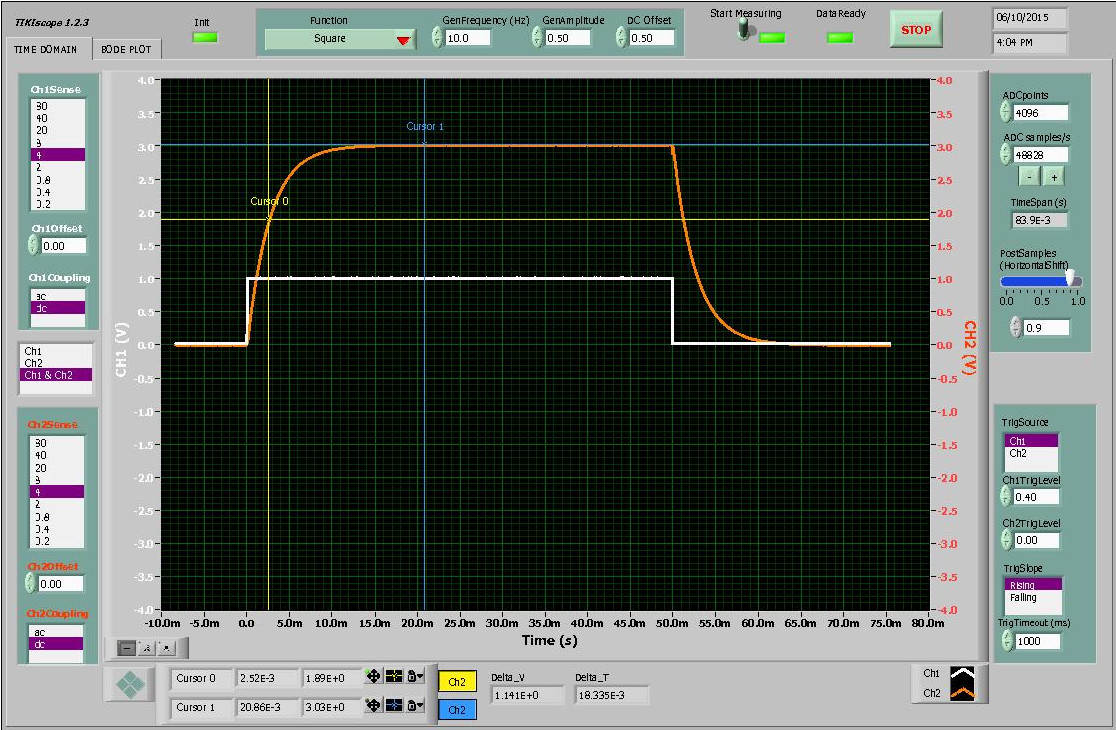
\includegraphics[width=7in]{TimeConstantOpen.jpg}
\caption{Time constant for open-loop configuration}
\label{fig:time-open}
\end{figure}

\begin{figure}[ht]
\centering
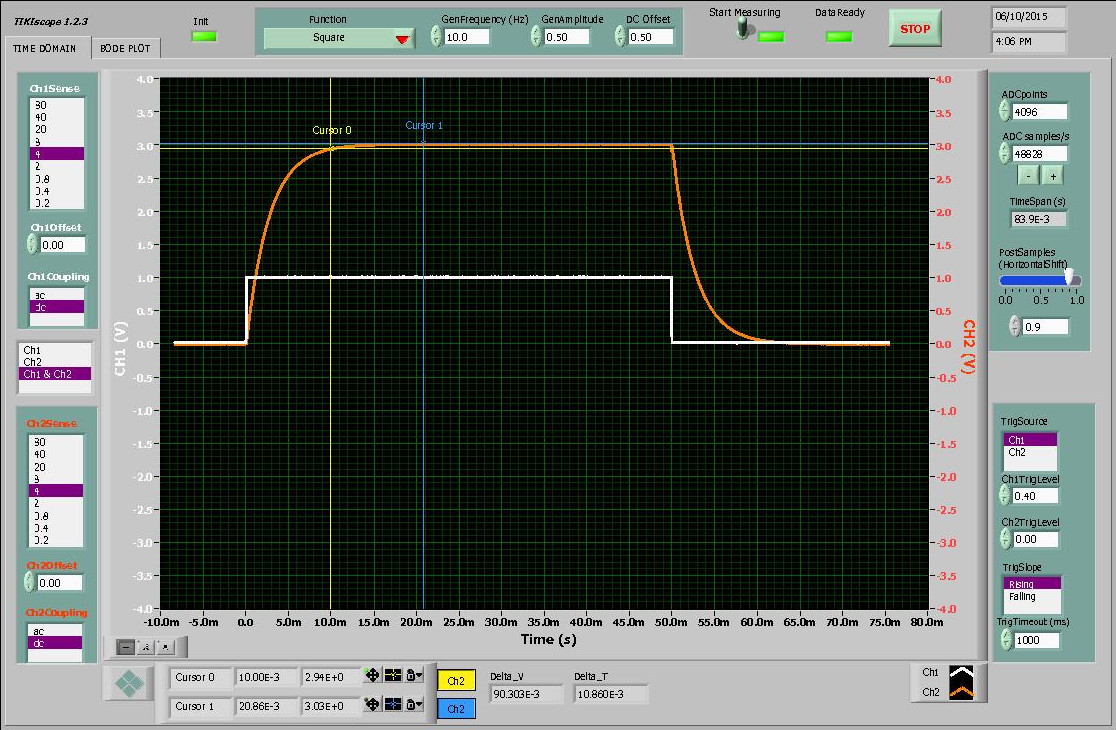
\includegraphics[width=7in]{SettlingOpen.jpg}
\caption{Settling time for open-loop configuration}
\label{fig:settle-open}
\end{figure}

\begin{figure}[ht]
\centering
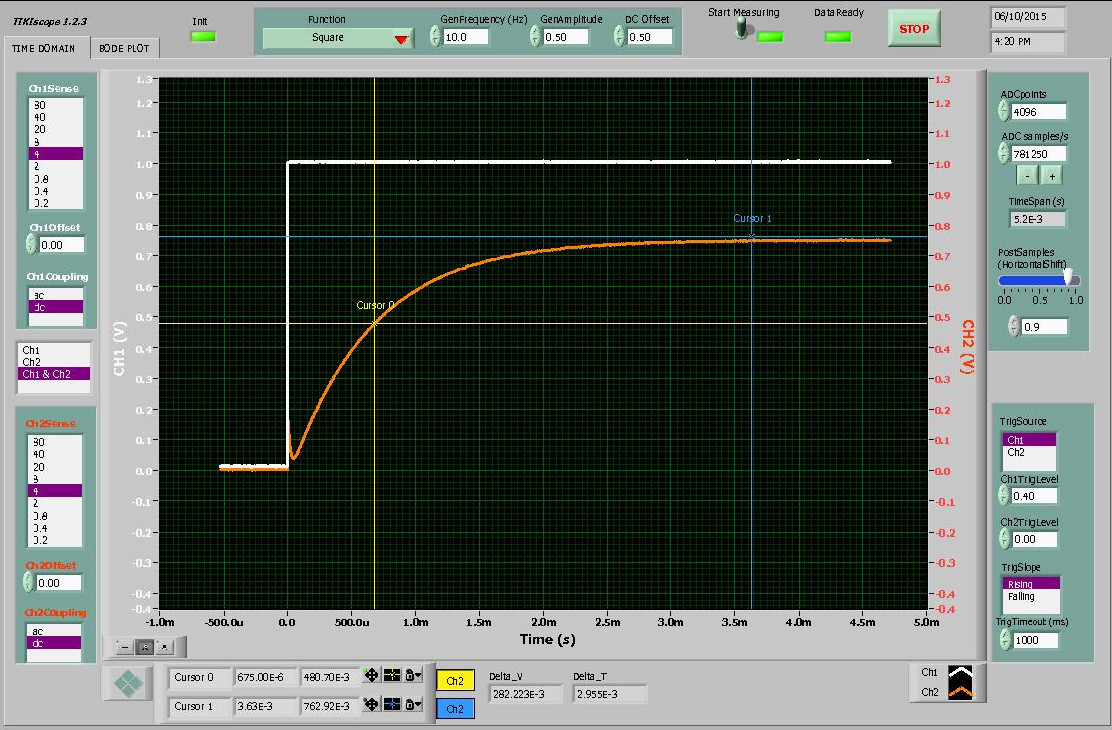
\includegraphics[width=7in]{TimeConstantClosed.jpg}
\caption{Time constant for closed-loop configuration}
\label{fig:time-closed}
\end{figure}

\begin{figure}[ht]
\centering
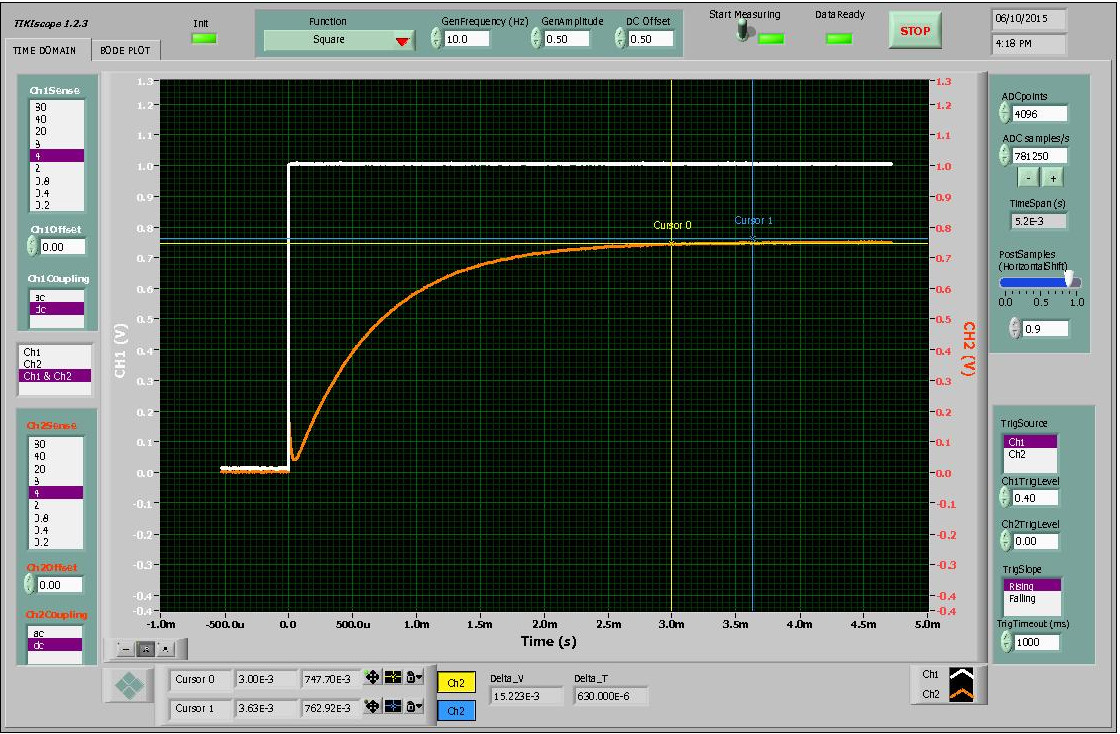
\includegraphics[width=7in]{SettlingClosed.jpg}
\caption{Settling time for closed-loop configuration}
\label{fig:settle-closed}
\end{figure}

\begin{figure}[ht]
\centering
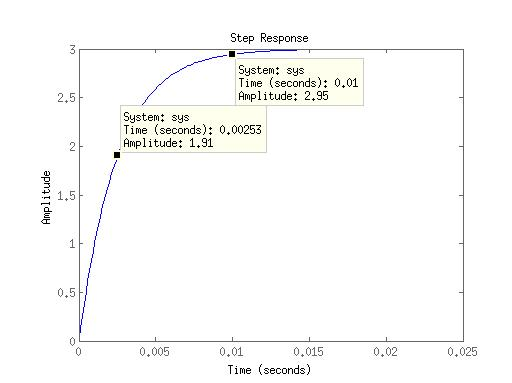
\includegraphics[width=7in]{MatlabFreqRespOpen.jpg}
\caption{Matlab Open-loop configuration}
\label{fig:matlab-open-loop}
\end{figure}


\begin{figure}[ht]
\centering
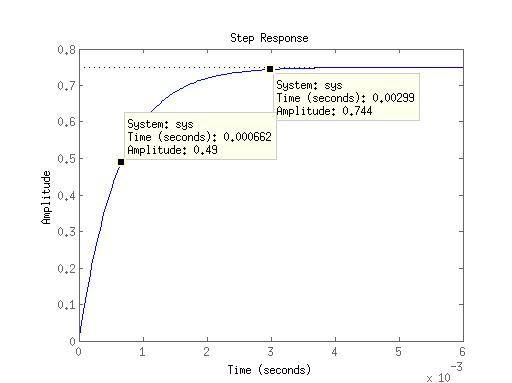
\includegraphics[width=7in]{MatlabFreqRespClosed.jpg}
\caption{Matlab Closed-loop configuration}
\label{fig:matlab-closed-loop}
\end{figure}

\begin{table}[ht]
\centering
    \begin{tabular}{|l|p{3cm}|p{3cm}|p{3cm}|p{3cm}|}
        \hline
        & \textbf{Tau Experimental} & \textbf{Tau Matlab} & \textbf{Tau Theoretical} & \textbf{Tau Error Theoretical vs Exerimental (\%)}\\
        \hline
        \textbf{Open-loop} & 2.50E-003 & 2.53E-003 & 2.50E-003 & 0\%\\
        \hline
        \textbf{Closed-loop} & 675E-006  & 662E-006 & 666.67E-006 & 0.002\%\\
        \hline
    \end{tabular}
    \caption{Summary of time-constant results}
    \label{tab:tau-summary}
\end{table}


\paragraph{Table 4 Discussion} % (fold)
\label{par:table_4_discussion}
The time constant is much smaller for a closed-loop system due to the stabilizing nature of a closed-loop system. Due to the output being fed into the input of the system, a closed loop system reaches its stable output much more quickly resulting in a lower time constant. The input function is now much larger and climbs faster allowing it to reach a portion of the output much faster.
% paragraph table_4_discussion (end)

\begin{table}[ht]
\centering
    \begin{tabular}{|l|p{3cm}|p{3cm}|p{3cm}|p{3cm}|}
        \hline
        & \textbf{Tau Experimental} & \textbf{Tau Matlab} & \textbf{Tau Theoretical} & \textbf{Tau Error Theoretical vs Exerimental (\%)}\\
        \hline
        \textbf{Open-loop} & 10.00E-003 & 10.0E-003 & 9.78E-003 & 0.22\%\\
        \hline
        \textbf{Closed-loop} & 3.00E-003 & 2.99E-003 & 2.45E-003 & 6.3\%\\
        \hline
    \end{tabular}
    \caption{Summary of 2\% settling time results}
    \label{tab:settle-summary}
\end{table}

\paragraph{Table 5 Discussion} % (fold)
\label{par:table_5_discussion}
Since settling time is the time it takes to reach a portion of the steady state value of the system, a closed-loop system whose input function is much larger due to the addition of the output function will reach its steady state much faster. This is also due to the input signal of a closed-loop system being very similar to the output signal, allowing them to match quickly.
% paragraph table_5_discussion (end)

\paragraph{Clipping} % (fold)
\label{par:clipping}
Clipping was observed at a value of $K_p = 28$ resulting in a clipped amplitude of 24.78V. This was possibly due to limitations of the signal generator (such as limitations on possible voltage generated) or the signal generation software (overflow errors in the software).
% paragraph clipping (end)


\end{document}
